%%% LaTeX Template: Two column article
%%%
%%% Source: http://www.howtotex.com/
%%% Feel free to distribute this template, but please keep to referal to http://www.howtotex.com/ here.
%%% Date: February 2011

%%% Preamble
\documentclass[	DIV=calc,%
							paper=a4,%
							fontsize=12pt,%
							onecolumn]{scrartcl}	 					% KOMA-article class

\usepackage{lipsum}													% Package to create dummy text
\usepackage[brazil]{babel}										% English language/hyphenation
\usepackage[protrusion=true,expansion=true]{microtype}				% Better typography
\usepackage{amsmath,amsfonts,amsthm}					% Math packages
\usepackage[pdftex]{graphicx}									% Enable pdflatex
\usepackage[svgnames]{xcolor}									% Enabling colors by their 'svgnames'
\usepackage[hang, small,labelfont=bf,up,textfont=it,up]{caption}	% Custom captions under/above floats
\usepackage{epstopdf}												% Converts .eps to .pdf
\usepackage{subfig}													% Subfigures
\usepackage{booktabs}												% Nicer tables
\usepackage{fix-cm}													% Custom fontsizes
\usepackage[utf8]{inputenc}
\usepackage[top=2.5cm, bottom=2.5cm, left=2.5cm, right=2.5cm]{geometry}
\usepackage[ddmmyyyy]{datetime}
\addto\captionsenglish{%
	\renewcommand\tablename{Tabela}
	\renewcommand\figurename{Figura}
} 
 

 
%%% Custom sectioning (sectsty package)
\usepackage{sectsty}													% Custom sectioning (see below)
\allsectionsfont{%															% Change font of al section commands
	\usefont{OT1}{phv}{b}{n}%										% bch-b-n: CharterBT-Bold font
	}

\sectionfont{%																% Change font of \section command
	\usefont{OT1}{phv}{b}{n}%										% bch-b-n: CharterBT-Bold font
	}



%%% Headers and footers
\usepackage{fancyhdr}												% Needed to define custom headers/footers
	\pagestyle{fancy}														% Enabling the custom headers/footers
\usepackage{lastpage}	

% Header (empty)
\lhead{}
\chead{}
\rhead{}
% Footer (you may change this to your own needs)

%% ====================================
%% ====================================
%% mude o rodape  do projeto
%% ====================================
%% ====================================

\lfoot{\footnotesize \texttt{Processo de Software} \textbullet ~Atividade 4}


\cfoot{}
\rfoot{\footnotesize página \thepage\ de \pageref{LastPage}}	% "Page 1 of 2"
\renewcommand{\headrulewidth}{0.0pt}
\renewcommand{\footrulewidth}{0.4pt}



%%% Creating an initial of the very first character of the content
\usepackage{lettrine}
\newcommand{\initial}[1]{%
     \lettrine[lines=3,lhang=0.3,nindent=0em]{
     				\color{DarkGoldenrod}
     				{\textsf{#1}}}{}}



%%% Title, author and date metadata
\usepackage{titling}															% For custom titles

\newcommand{\HorRule}{\color{DarkGoldenrod}%			% Creating a horizontal rule
									  	\rule{\linewidth}{1pt}%
										}

\pretitle{\vspace{-30pt} \begin{flushleft} \HorRule 
				\fontsize{50}{50} \usefont{OT1}{phv}{b}{n} \color{DarkRed} \selectfont 
				}

%% ====================================
%% ====================================
%% mude o titulo  do projeto
%% ====================================
%% ====================================

\title{Relatório de Desenvolvimento do Processo de Software}					% Title of your article goes here

%% ====================================



\posttitle{\par\end{flushleft}\vskip 0.5em}

\preauthor{\begin{flushleft}
					\large \lineskip 0.5em \usefont{OT1}{phv}{b}{sl} \color{DarkRed}}
\author{Giovana Carolina de Gois}  	% Author name goes here


\postauthor{\footnotesize \usefont{OT1}{phv}{m}{sl} \color{Black} 
					\\Universidade Tecnológica Federal do Paraná - Câmpus Cornélio Procópio 								% Institution of author
					\par\end{flushleft}\HorRule}

\date{}																				% No date




%%% Begin document
\begin{document}
\maketitle
\thispagestyle{fancy} 	
\thispagestyle{empty}		% Enabling the custom headers/footers for the first page 
% The first character should be within \initial{}




%% ====================================
%% ====================================
%% mude o resumo  do projeto
%% ====================================
%% ====================================
\initial{E}\textbf{ste documento apresenta o detalhamento do processo de software de uma empresa de Desenvolvimento Web voltada à criação de sites. O cenário representado é composto por sete colaboradores. Os clientes são empresas e profissionais que desejam incluir seu negócio ou serviço na esfera digital, que ainda não possuem uma \textit{landing page}. O estudo desse cenário foi desenvolvido por constatar que em grande parte das vezes esse tipo de produto é produzido ``informalmente", sem realizar controle do processo.}


%% ====================================
\begin{figure}
	\centering
	
\includegraphics{utfpr}
\end{figure}

\vspace{3cm}
\centerline{\textit{\textbf{\today}}}

\clearpage
    \renewcommand*\listfigurename{Lista de figuras}
\listoffigures

\renewcommand*\listtablename{Lista de tabelas}
\listoftables




\clearpage
\renewcommand{\contentsname}{Sumário}
\tableofcontents
\clearpage

%% ====================================
%% ====================================
%% Inicio do texto
%% ====================================
%% ====================================
\section{Introdução}
Este trabalho tem por objetivo ilustrar o processo de desenvolvimento de software utilizado numa empresa fictícia de desenvolvimento voltado à web, mais especificamente, websites profissionais. O rol de clientes pode ser definido como sendo composto por empresas ou profissionais liberais que desejem estar digitalmente presentes através da criação de websites. 
O processo basicamente se resume em:
\begin{itemize}
	\item Cliente procura a empresa;
	\item Empresa propõe um protótipo e realiza orçamento;
	\item Negociam formas de pagamento;
	\item Desenvolvimento com entregas parciais, quando aplicável;
	\item Contato com suporte para orientações;
	\item Realização da entrega e pagamento.
\end{itemize}


\section{Processo}
Para melhor visualização, o processo foi dividido em dois diagramas: o primeiro ilustrando a coleta de requisitos e aprovação do cliente, e o segundo representando a etapa de construção do produto.

\subsection{Papeis}
Os seguintes papeis estão envolvidos no processo:
\begin{itemize}
	\item Cliente;
	\item Analista de Atendimento ao Cliente;
	\item Analista de Requisitos;
	\item Equipe de Desenvolvimento (pelo menos 2 pessoas);
	\item Analista de Suporte;
	\item Designer de Interfaces.
\end{itemize}


\subsection{Execução do projeto}

Para melhor visualização, o processo foi dividido em duas etapas: (i) Abordagem e Coleta de Requisitos e (ii) Desenvolvimento do Projeto.

\subsubsection{Abordagem e Coleta de Requisitos}

A Figura \ref{diag_requisitos} apresenta a primeira etapa do processo, partindo da primeira atividade: o primeiro contato com o Cliente. A solicitação é atendida por um colaborador da área de Atendimento ao Cliente, que encaminha a solicitação inicial ao Analista de Requisitos. O Analista de Requisitos fica responsável por levantar as necessidades do Cliente e produzir, junto ao Designer, um ou mais protótipos da interface para aprovação do Cliente. O departamento Financeiro também é informado sobre os dados do projeto para que possa formalizar o orçamento. É realizada uma reunião com o cliente para apresentação dos protótipos e negociação do orçamento. Após finalizado, o Analista de Requisitos elabora as documentações que servirão de base para a etapa de Desenvolvimento. 

\begin{figure}[!h]
	\caption{Etapa I - Abordagem e Coleta de Requisitos}
	\centering
	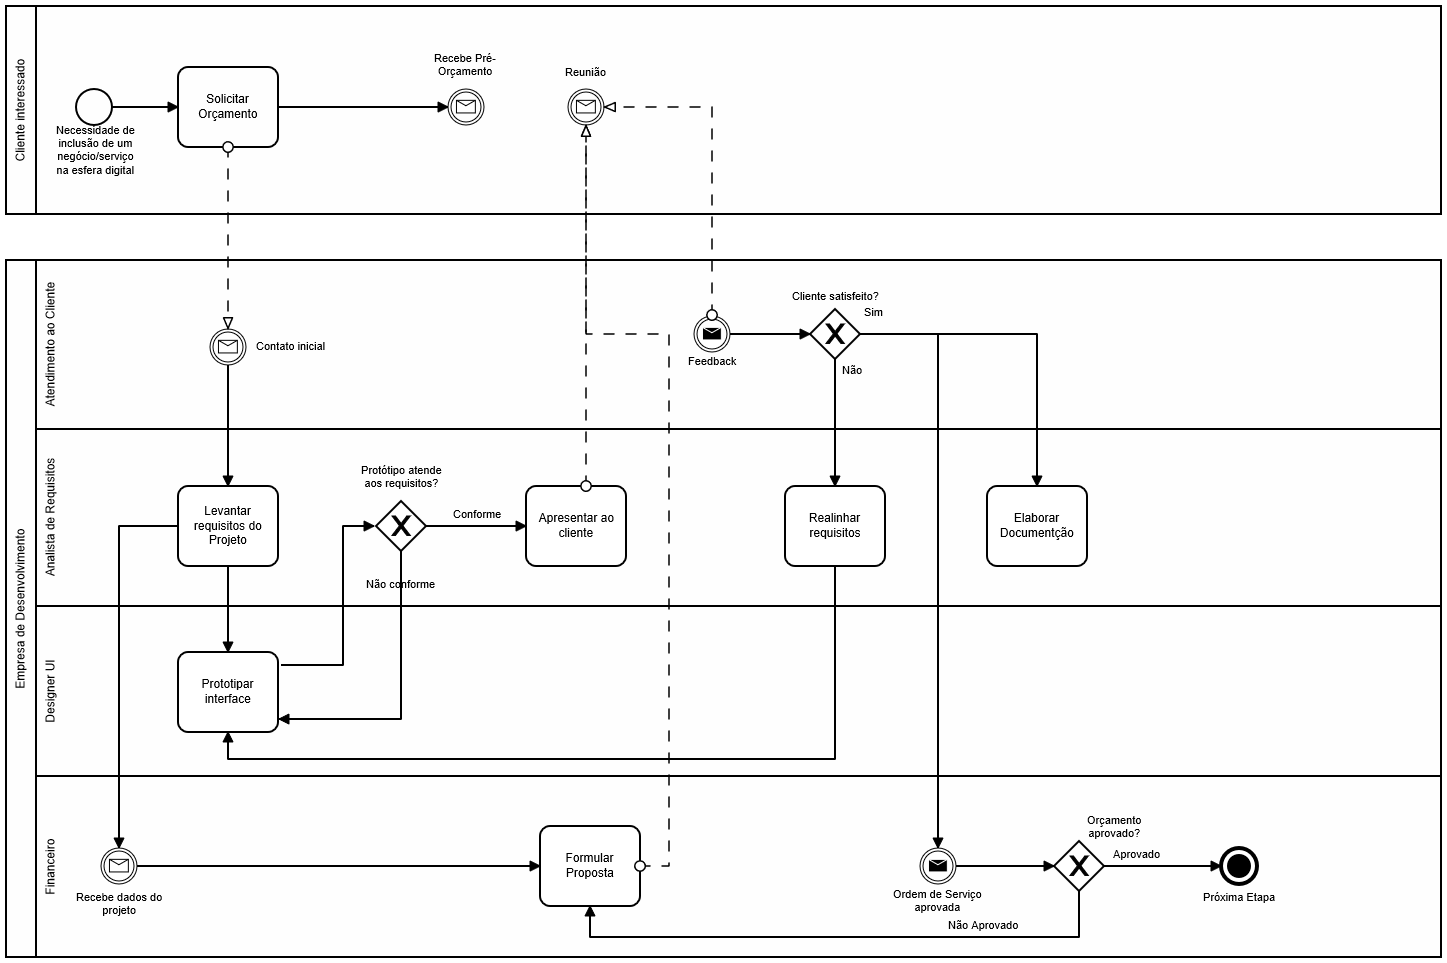
\includegraphics[width=\textwidth]{Requisitos}
	{Fonte: Autoria Própria. Modelagem: https://bpmn.io/}
\end{figure}\label{diag_requisitos}

\subsubsection{Desenvolvimento do Produto de Software}
 
A Figura \ref{diag_desenvolvimento} representa a etapa de desenvolvimento do projeto de software. Nela, o analista de requisitos fornece a documentação para que a equipe de desenvolvimento possa definir a abordagem e iniciar a produção dos artefatos. Uma vez iniciada, é cumprida a etapa de testes e validação dos requisitos antes de apresentar um artefato ao Cliente. Se aprovado, a produção do próximo incremento se inicia, do contrário, o \textit{feedback} é documentado e a equipe realiza as alterações necessárias. Ao finalizar, o departamento Financeiro é avisado para que o pedido seja faturado e negociado com o Cliente. A entrega é realizada e o departamento de Suporte fica à disposição para eventuais orientações.

\begin{figure}
	\caption{Etapa II - Desenvolvimento do Produto}
	\centering
	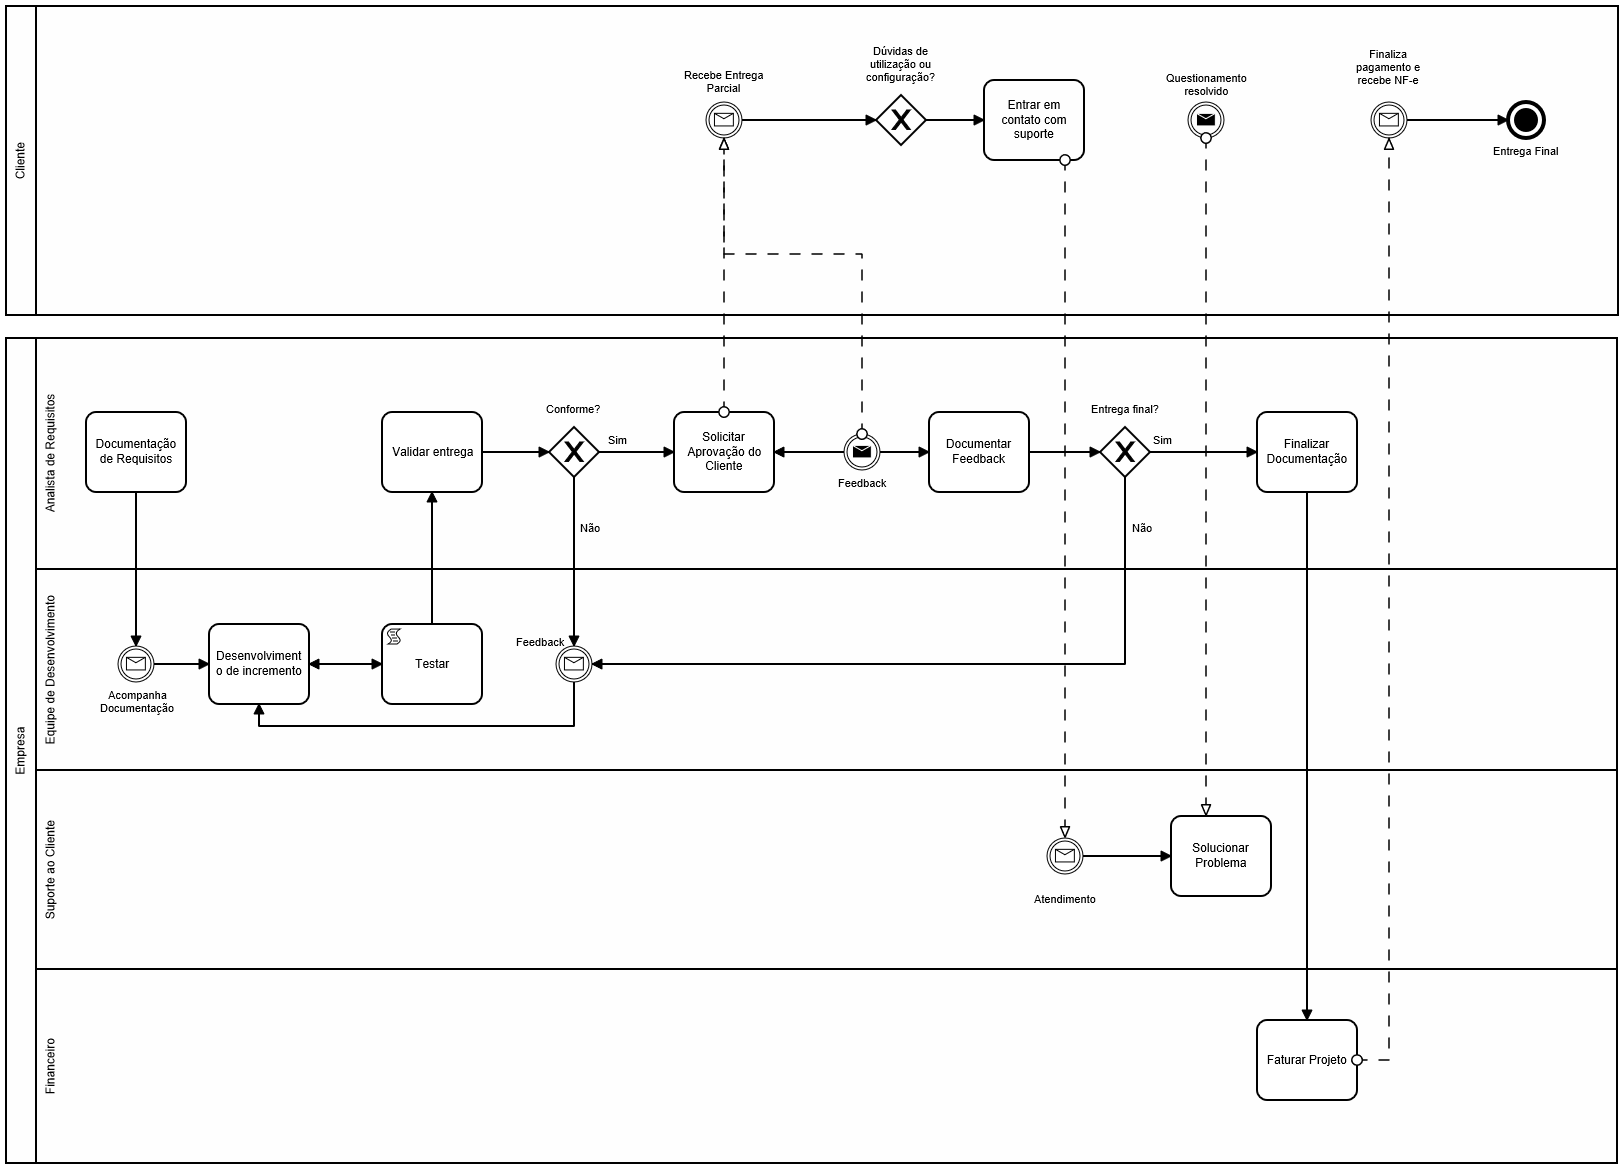
\includegraphics[width=\textwidth]{Desenvolvimento}
	{Fonte: Autoria Própria. Modelagem: https://bpmn.io/}
\end{figure}\label{diag_desenvolvimento}


\renewcommand\refname{} %%Referências bibliográficas}  
\bibliographystyle{ieeetr}
\bibliography{referencias}  

\end{document}